\documentclass[]{article}
\usepackage{lmodern}
\usepackage{amssymb,amsmath}
\usepackage{ifxetex,ifluatex}
\usepackage{fixltx2e} % provides \textsubscript
\ifnum 0\ifxetex 1\fi\ifluatex 1\fi=0 % if pdftex
  \usepackage[T1]{fontenc}
  \usepackage[utf8]{inputenc}
\else % if luatex or xelatex
  \ifxetex
    \usepackage{mathspec}
  \else
    \usepackage{fontspec}
  \fi
  \defaultfontfeatures{Ligatures=TeX,Scale=MatchLowercase}
\fi
% use upquote if available, for straight quotes in verbatim environments
\IfFileExists{upquote.sty}{\usepackage{upquote}}{}
% use microtype if available
\IfFileExists{microtype.sty}{%
\usepackage{microtype}
\UseMicrotypeSet[protrusion]{basicmath} % disable protrusion for tt fonts
}{}
\usepackage[margin=1in]{geometry}
\usepackage{hyperref}
\hypersetup{unicode=true,
            pdftitle={A Predictive Model for Life Expectancy},
            pdfauthor={Rachel Tsong and Adina Zhang},
            pdfborder={0 0 0},
            breaklinks=true}
\urlstyle{same}  % don't use monospace font for urls
\usepackage{color}
\usepackage{fancyvrb}
\newcommand{\VerbBar}{|}
\newcommand{\VERB}{\Verb[commandchars=\\\{\}]}
\DefineVerbatimEnvironment{Highlighting}{Verbatim}{commandchars=\\\{\}}
% Add ',fontsize=\small' for more characters per line
\usepackage{framed}
\definecolor{shadecolor}{RGB}{248,248,248}
\newenvironment{Shaded}{\begin{snugshade}}{\end{snugshade}}
\newcommand{\KeywordTok}[1]{\textcolor[rgb]{0.13,0.29,0.53}{\textbf{#1}}}
\newcommand{\DataTypeTok}[1]{\textcolor[rgb]{0.13,0.29,0.53}{#1}}
\newcommand{\DecValTok}[1]{\textcolor[rgb]{0.00,0.00,0.81}{#1}}
\newcommand{\BaseNTok}[1]{\textcolor[rgb]{0.00,0.00,0.81}{#1}}
\newcommand{\FloatTok}[1]{\textcolor[rgb]{0.00,0.00,0.81}{#1}}
\newcommand{\ConstantTok}[1]{\textcolor[rgb]{0.00,0.00,0.00}{#1}}
\newcommand{\CharTok}[1]{\textcolor[rgb]{0.31,0.60,0.02}{#1}}
\newcommand{\SpecialCharTok}[1]{\textcolor[rgb]{0.00,0.00,0.00}{#1}}
\newcommand{\StringTok}[1]{\textcolor[rgb]{0.31,0.60,0.02}{#1}}
\newcommand{\VerbatimStringTok}[1]{\textcolor[rgb]{0.31,0.60,0.02}{#1}}
\newcommand{\SpecialStringTok}[1]{\textcolor[rgb]{0.31,0.60,0.02}{#1}}
\newcommand{\ImportTok}[1]{#1}
\newcommand{\CommentTok}[1]{\textcolor[rgb]{0.56,0.35,0.01}{\textit{#1}}}
\newcommand{\DocumentationTok}[1]{\textcolor[rgb]{0.56,0.35,0.01}{\textbf{\textit{#1}}}}
\newcommand{\AnnotationTok}[1]{\textcolor[rgb]{0.56,0.35,0.01}{\textbf{\textit{#1}}}}
\newcommand{\CommentVarTok}[1]{\textcolor[rgb]{0.56,0.35,0.01}{\textbf{\textit{#1}}}}
\newcommand{\OtherTok}[1]{\textcolor[rgb]{0.56,0.35,0.01}{#1}}
\newcommand{\FunctionTok}[1]{\textcolor[rgb]{0.00,0.00,0.00}{#1}}
\newcommand{\VariableTok}[1]{\textcolor[rgb]{0.00,0.00,0.00}{#1}}
\newcommand{\ControlFlowTok}[1]{\textcolor[rgb]{0.13,0.29,0.53}{\textbf{#1}}}
\newcommand{\OperatorTok}[1]{\textcolor[rgb]{0.81,0.36,0.00}{\textbf{#1}}}
\newcommand{\BuiltInTok}[1]{#1}
\newcommand{\ExtensionTok}[1]{#1}
\newcommand{\PreprocessorTok}[1]{\textcolor[rgb]{0.56,0.35,0.01}{\textit{#1}}}
\newcommand{\AttributeTok}[1]{\textcolor[rgb]{0.77,0.63,0.00}{#1}}
\newcommand{\RegionMarkerTok}[1]{#1}
\newcommand{\InformationTok}[1]{\textcolor[rgb]{0.56,0.35,0.01}{\textbf{\textit{#1}}}}
\newcommand{\WarningTok}[1]{\textcolor[rgb]{0.56,0.35,0.01}{\textbf{\textit{#1}}}}
\newcommand{\AlertTok}[1]{\textcolor[rgb]{0.94,0.16,0.16}{#1}}
\newcommand{\ErrorTok}[1]{\textcolor[rgb]{0.64,0.00,0.00}{\textbf{#1}}}
\newcommand{\NormalTok}[1]{#1}
\usepackage{graphicx,grffile}
\makeatletter
\def\maxwidth{\ifdim\Gin@nat@width>\linewidth\linewidth\else\Gin@nat@width\fi}
\def\maxheight{\ifdim\Gin@nat@height>\textheight\textheight\else\Gin@nat@height\fi}
\makeatother
% Scale images if necessary, so that they will not overflow the page
% margins by default, and it is still possible to overwrite the defaults
% using explicit options in \includegraphics[width, height, ...]{}
\setkeys{Gin}{width=\maxwidth,height=\maxheight,keepaspectratio}
\IfFileExists{parskip.sty}{%
\usepackage{parskip}
}{% else
\setlength{\parindent}{0pt}
\setlength{\parskip}{6pt plus 2pt minus 1pt}
}
\setlength{\emergencystretch}{3em}  % prevent overfull lines
\providecommand{\tightlist}{%
  \setlength{\itemsep}{0pt}\setlength{\parskip}{0pt}}
\setcounter{secnumdepth}{0}
% Redefines (sub)paragraphs to behave more like sections
\ifx\paragraph\undefined\else
\let\oldparagraph\paragraph
\renewcommand{\paragraph}[1]{\oldparagraph{#1}\mbox{}}
\fi
\ifx\subparagraph\undefined\else
\let\oldsubparagraph\subparagraph
\renewcommand{\subparagraph}[1]{\oldsubparagraph{#1}\mbox{}}
\fi

%%% Use protect on footnotes to avoid problems with footnotes in titles
\let\rmarkdownfootnote\footnote%
\def\footnote{\protect\rmarkdownfootnote}

%%% Change title format to be more compact
\usepackage{titling}

% Create subtitle command for use in maketitle
\providecommand{\subtitle}[1]{
  \posttitle{
    \begin{center}\large#1\end{center}
    }
}

\setlength{\droptitle}{-2em}

  \title{A Predictive Model for Life Expectancy}
    \pretitle{\vspace{\droptitle}\centering\huge}
  \posttitle{\par}
    \author{Rachel Tsong and Adina Zhang}
    \preauthor{\centering\large\emph}
  \postauthor{\par}
      \predate{\centering\large\emph}
  \postdate{\par}
    \date{April 7, 2019}


\begin{document}
\maketitle

\subsection{Introduction}\label{introduction}

\subsubsection{Motivation}\label{motivation}

The dataset for our analysis was compiled by the Global Health
Observatory (GHO), a branch of the World Health Organization (WHO). The
repository contains data collected from 2000 to 2015 from 193 countries
about factors relating to life expectancy. These factors include
mortality rates of adults as well as infants and children, economic
factors such as GDP and government health expenditures, disease related
data such as incidence of measles and HIV, and health related variables
such as BMI and alcohol consumption. Our analysis aims to answer the
following questions:

\begin{itemize}
\tightlist
\item
  Which covariates are most predictive of life expectancy?
\item
  What modeling method most accurately predicts life expectancy?
\end{itemize}

The results of analyses such as ours can be used by governments to
direct resources and health care expenditures on the variables that are
most strongly associated with life expectancy in order to improve the
population's longevity and livelihood.

\subsubsection{Data Cleaning}\label{data-cleaning}

The original data set has 22 variables and 2938 observations from 193
countries between 2000 and 2015. A correlation matrix was used to assess
the predictors to determine if there were any highly correlated
variables. In order to avoid multicollinearity and to create a more
parsimonious model, highly correlated variables were removed. Among the
variables removed were infant deaths, percentage expenditure, measles,
polio, and thinness for children ages 5 to 9 years. Population was also
removed from the dataset because it is not an appropriate standardized
measurement for life expectancy. Without adjusting population for area
it is not a good comparative measurement. One dichotomous variable in
our dataset that describes development status was recoded into an
integer with groups 0 and 1. Any entries with NAs were omitted. The
final analysis dataset has 15 variables with 1853 observations.

\subsection{EDA}\label{eda}

In exploratory data analysis, one of the main goals was to characterize
the relationship of predictors with life expectancy. From the
scatterplot in the figure below, we were able to conclude that several
predictors potentially have a non-linear relationship with life
expectancy. These predictors include GDP, thinness of children ages
1-19, BMI, total expenditure, diphtheria, HIV/AIDS, adult mortality,
alcohol, and hepatitis B.

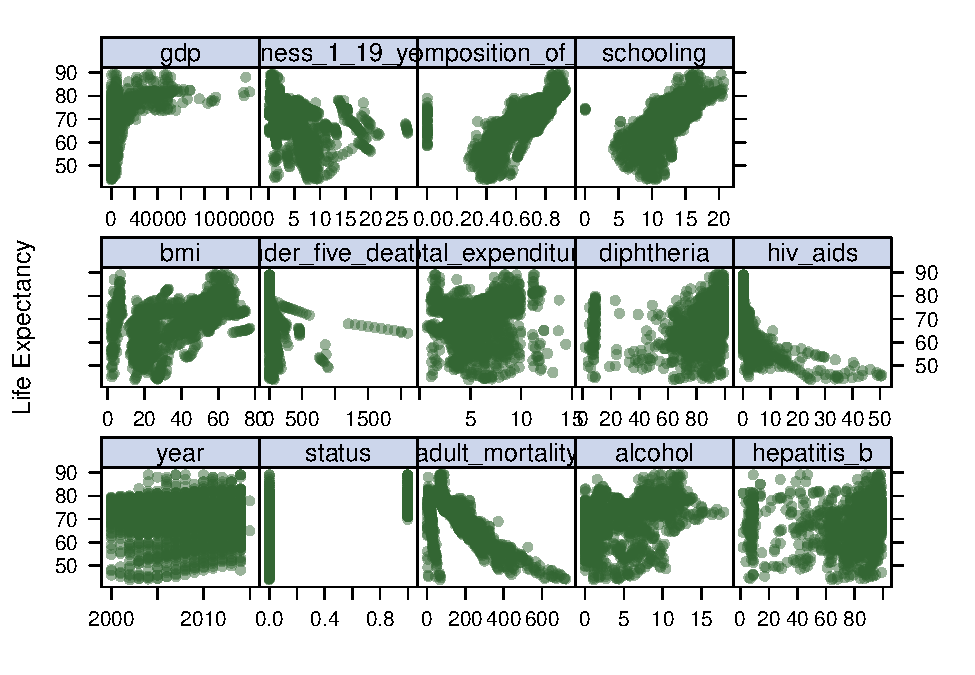
\includegraphics{midterm_project_report_files/figure-latex/unnamed-chunk-2-1.pdf}

\subsection{Model Building}\label{model-building}

\subsubsection{Method}\label{method}

The data was split into training and test sets through 10-fold cross
validation. Four models were fit using the training data including least
squares, Lasso, GAM, and MARS. Tuning parameters for Lasso and MARS were
chosen through cross validation. To compare model results, the fitted
models were used for prediction on the teting sets and RMSE was
calculated for comparison.

\subsubsection{Variables}\label{variables}

The reduced dataset contained 14 possible predictors for
\texttt{life\_expectancy} in years: \texttt{year}, \texttt{status} (a
binary variable with 0 = developing and 1 = developed),
\texttt{adult\_mortality} (number of deaths per 1000 people aged 15-60),
\texttt{alcohol} (average liters of alcohol consumed per capita),
\texttt{hepatitis\_b} (percent of 1 year olds immunized against Hep B),
\texttt{bmi}, \texttt{under\_five\_deaths} (number of under 5 deaths per
1000), \texttt{total\_expenditure} (percentage of government spending on
health), \texttt{diphtheria} (percent of 1 year olds immunized againt
diphtheria), \texttt{hiv\_aids} (deaths from HIV/AIDS per 1000 among 0-4
year olds), \texttt{gdp}, \texttt{thinness\_1\_19\_years} (prevalence of
thinness among 1-19 year olds),
\texttt{income\_composition\_of\_resources} (human development index
measure of income composition), and \texttt{schooling} (number of
years).

\subsubsection{Linear Models}\label{linear-models}

First, we fit ordinary least squares regression and Lasso regression. We
chose these because they are widely used and easily interpretable; but
because it seemed as if there were many non-linear relationships we did
not necessarily expect these models to fit the data the best. However,
they provided baseline RMSEs that we could compare other models to. The
assumptions for these types of regressions are linearity in parameters,
homoscedasticity, and errors that are normal and uncorrelated. In our
least squares model fit all predictors were significant at the 5\% level
except alcohol, hepatitis B, and under five deaths. The covariates that
were more predictive of life expectancy (meaning their coefficients were
large and the p-value for the estimates were small) were adult ortality
and income composition of resources. For the Lasso fit, an optimal
lambda was chosen by cross-validation, and only hepatitis B was shrunk
to zero. Similarly to the least squares model, adult mortality and
income composition of resources were most predictive of life expectancy.
After 10-fold cross-validation was performed on the test sets, mean
RMSEs for least squares and Lasso were 3.73 and 3.74, respectively.
These models, though easily interpetable, lack flexibility as they
cannot account for non-linear variables. In the next sections, we
discuss two more models that have greater flexibility and might capture
the true relationship more accurately.

\subsubsection{GAM}\label{gam}

We fit a generalized additive model (GAM) using all the predictors with
smoothing splines on GDP, thinness of children ages 1-19, BMI, total
expenditure, diphtheria, HIV/AIDS, adult mortality, alcohol, and
hepatitis B. These variables were chosen because the correlation plots
appeared highly non-linear. Since we used the \texttt{mgcv::gam()}
function, we did not have to specify the degrees of freedom for the
splines. This model assumes additivity, thus important interaction terms
can be missed by this method; however, it is advantageous to linear
regression techniques because there can be both linear and non-linear
predictors; however, it is difficult to interpret non-linear
relationships. In our GAM fit, even when a smoothing spline was applied,
hepatitis B was still non-significant at the 5\% confidence level. As in
the linear models in the previous section income composition was an
important predictor of life expectancy. 10-fold cross-validation was
performed on testing data, and the mean RMSE was 2.99.

\subsubsection{MARS}\label{mars}

Lastly, we fit a multivariate adaptive regression spline (MARS) from the
\texttt{earth} package. The optimal maximum degree and number of terms
were chosen by cross-validation. The MARS model is advantageous because
it is highly flexible yet still interpretable. The relationships between
covariate and outcome are linear, but the model fits knots to account
for non-constant slopes, and the model can take into account interaction
terms. In our MARS model, only 6 predictors were kept in the model. In
decreasing order of importance the variables were income composition,
HIV/AIDS, adult mortality, under five deaths, and thinness 1-19 years.
Additionally, 1 knot was created for adult mortality, under five deaths,
HIV/AIDS, and thinness, indicating that these predictors have a
non-constant relationship to life expectancy. The model added 17
interaction terms, suggesting that many of the predictors have effects
on the others. After subsetting the data into test and training sets,
10-fold cross validation was performed, and the mean RMSE was found to
be 2.09.

\subsubsection{Model Comparison}\label{model-comparison}

The results of 10-fold cross validation are shown in the figure below.
Both GAM and MARS had significantly lower RMSEs than either least
squares or lasso regression which performed similarly. Ultimately, MARS
fit the best model as it has the lowest RMSE. As discussed previously,
the reasons why GAM and MARS perform better is because they allow
flexibility for non-parametric variables. MARS outperforms GAM because
the method takes into account any interaction terms that exist and it
eliminates any variables not deemed significant to the outcome, thereby
creating a more parsimonious model.

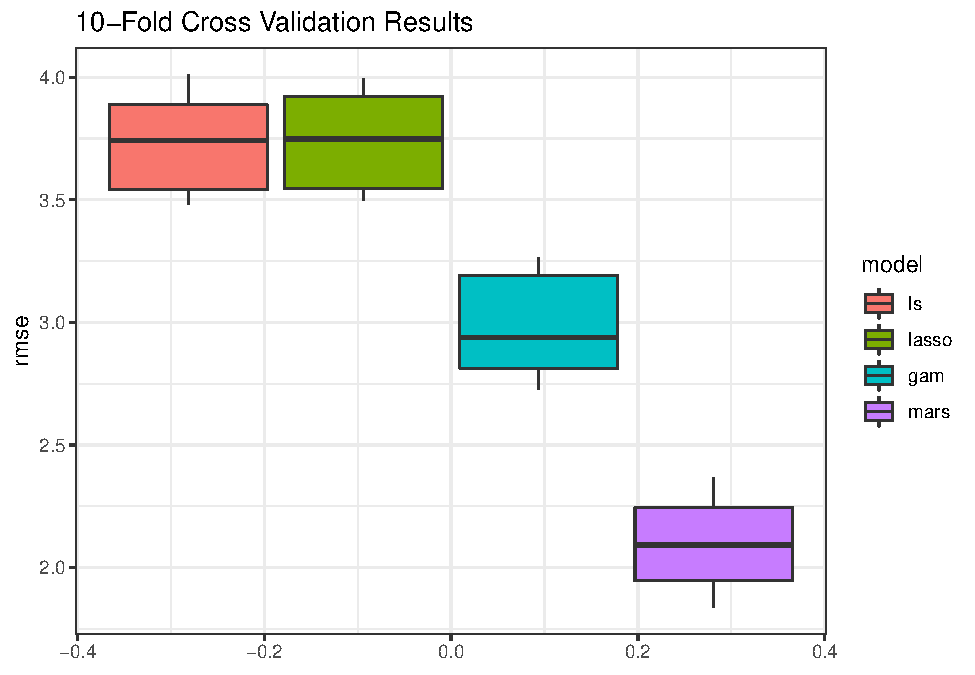
\includegraphics{midterm_project_report_files/figure-latex/unnamed-chunk-4-1.pdf}

\subsection{Conclusions}\label{conclusions}

From our analysis, it was determined that the best model to predict life
expectancy was the MARS method. This method offered both flexibility
when handling non-parameteric variables and a parsimonious model.
Furthermore, the MARS method takes into account interaction terms that
may exist which is ignored in the GAM method. When it came to predicting
life expectancy and understanding which parameters were most significant
in prediction, income composition of resources was consistently
important in least squares, lasso, and MARs.

\newpage

\subsection{Appendix}\label{appendix}

\paragraph{Data Cleaning}\label{data-cleaning-1}

\begin{Shaded}
\begin{Highlighting}[]
\CommentTok{# Load dataset}
\NormalTok{life_analysis =}\StringTok{ }\KeywordTok{read_csv}\NormalTok{(}\StringTok{"./Life Expectancy Data.csv"}\NormalTok{) }\OperatorTok\StringTok{ }
\StringTok{  }\NormalTok{janitor}\OperatorTok{::}\KeywordTok{clean_names}\NormalTok{() }\OperatorTok
\StringTok{  }\KeywordTok{select}\NormalTok{(}\OperatorTok{-}\NormalTok{country, }\OperatorTok{-}\NormalTok{population, }\OperatorTok{-}\NormalTok{infant_deaths, }\OperatorTok{-}\NormalTok{measles, }
         \OperatorTok{-}\NormalTok{polio, }\OperatorTok{-}\NormalTok{thinness_5_9_years, }\OperatorTok{-}\NormalTok{percentage_expenditure) }\OperatorTok\StringTok{ }
\StringTok{  }\KeywordTok{mutate}\NormalTok{(}\DataTypeTok{status =} \KeywordTok{factor}\NormalTok{(status),}
         \DataTypeTok{status =} \KeywordTok{fct_recode}\NormalTok{(status, }\StringTok{"0"}\NormalTok{ =}\StringTok{ "Developing"}\NormalTok{, }\StringTok{"1"}\NormalTok{ =}\StringTok{ "Developed"}\NormalTok{),}
         \DataTypeTok{status =} \KeywordTok{ifelse}\NormalTok{(status }\OperatorTok{==}\StringTok{ "1"}\NormalTok{, }\DecValTok{1}\NormalTok{, }\DecValTok{0}\NormalTok{)) }
\NormalTok{life_analysis =}\StringTok{ }\KeywordTok{na.omit}\NormalTok{(life_analysis)}
\end{Highlighting}
\end{Shaded}

\paragraph{Scatterplot}\label{scatterplot}

\begin{Shaded}
\begin{Highlighting}[]
\CommentTok{# Scatterplot}
\NormalTok{x =}\StringTok{ }\KeywordTok{model.matrix}\NormalTok{(life_expectancy }\OperatorTok{~}\NormalTok{., life_analysis)}
\NormalTok{y =}\StringTok{ }\NormalTok{life_analysis}\OperatorTok{$}\NormalTok{life_expectancy}

\NormalTok{theme1 <-}\StringTok{ }\KeywordTok{trellis.par.get}\NormalTok{()}
\NormalTok{theme1}\OperatorTok{$}\NormalTok{plot.symbol}\OperatorTok{$}\NormalTok{col <-}\StringTok{ }\KeywordTok{rgb}\NormalTok{(.}\DecValTok{2}\NormalTok{, .}\DecValTok{4}\NormalTok{, .}\DecValTok{2}\NormalTok{, .}\DecValTok{5}\NormalTok{)}
\NormalTok{theme1}\OperatorTok{$}\NormalTok{plot.symbol}\OperatorTok{$}\NormalTok{pch <-}\StringTok{ }\DecValTok{16}
\NormalTok{theme1}\OperatorTok{$}\NormalTok{strip.background}\OperatorTok{$}\NormalTok{col <-}\StringTok{ }\KeywordTok{rgb}\NormalTok{(.}\DecValTok{0}\NormalTok{, .}\DecValTok{2}\NormalTok{, .}\DecValTok{6}\NormalTok{, .}\DecValTok{2}\NormalTok{)}
\KeywordTok{trellis.par.set}\NormalTok{(theme1) }
\KeywordTok{featurePlot}\NormalTok{(x[,}\OperatorTok{-}\DecValTok{1}\NormalTok{], y, }\DataTypeTok{plot =} \StringTok{"scatter"}\NormalTok{, }\DataTypeTok{labels =} \KeywordTok{c}\NormalTok{(}\StringTok{""}\NormalTok{,}\StringTok{"Life Expectancy"}\NormalTok{))}
\end{Highlighting}
\end{Shaded}

\paragraph{Tuning parameters for Lasso and
MARS}\label{tuning-parameters-for-lasso-and-mars}

\begin{Shaded}
\begin{Highlighting}[]
\CommentTok{# Tuning parameters}

\CommentTok{# Tuning lambda for lasso through cross validation}
\KeywordTok{set.seed}\NormalTok{(}\DecValTok{123}\NormalTok{)}
\NormalTok{cv_lasso =}\StringTok{ }\KeywordTok{cv.glmnet}\NormalTok{(x, y, }\DataTypeTok{alpha =} \DecValTok{1}\NormalTok{)}
\NormalTok{best_lambda =}\StringTok{ }\NormalTok{cv_lasso}\OperatorTok{$}\NormalTok{lambda.min}
\KeywordTok{plot_glmnet}\NormalTok{(cv_lasso}\OperatorTok{$}\NormalTok{glmnet.fit)}

\CommentTok{# Tuning for MARS}
\CommentTok{# Create a tuning grid}
\NormalTok{hyper_grid =}\StringTok{ }\KeywordTok{expand.grid}\NormalTok{(}
  \DataTypeTok{degree =} \DecValTok{1}\OperatorTok{:}\DecValTok{3}\NormalTok{, }
  \DataTypeTok{nprune =} \KeywordTok{seq}\NormalTok{(}\DecValTok{2}\NormalTok{, }\DecValTok{70}\NormalTok{, }\DataTypeTok{length.out =} \DecValTok{20}\NormalTok{) }\OperatorTok\StringTok{ }\KeywordTok{floor}\NormalTok{()}
\NormalTok{  )}

\KeywordTok{set.seed}\NormalTok{(}\DecValTok{1}\NormalTok{)}
\CommentTok{# Cross validated model}
\NormalTok{tuned_mars =}\StringTok{ }\KeywordTok{train}\NormalTok{(}
  \DataTypeTok{x =} \KeywordTok{subset}\NormalTok{(life_analysis, }\DataTypeTok{select =} \OperatorTok{-}\NormalTok{life_expectancy),}
  \DataTypeTok{y =}\NormalTok{ life_analysis}\OperatorTok{$}\NormalTok{life_expectancy,}
  \DataTypeTok{method =} \StringTok{"earth"}\NormalTok{,}
  \DataTypeTok{metric =} \StringTok{"RMSE"}\NormalTok{,}
  \DataTypeTok{trControl =} \KeywordTok{trainControl}\NormalTok{(}\DataTypeTok{method =} \StringTok{"cv"}\NormalTok{, }\DataTypeTok{number =} \DecValTok{10}\NormalTok{),}
  \DataTypeTok{tuneGrid =}\NormalTok{ hyper_grid}
\NormalTok{)}

\CommentTok{# best model}
\NormalTok{tuned_mars}\OperatorTok{$}\NormalTok{bestTune}

\KeywordTok{ggplot}\NormalTok{(tuned_mars)}
\end{Highlighting}
\end{Shaded}

\paragraph{10-fold cross validation with four modeling
methods}\label{fold-cross-validation-with-four-modeling-methods}

\begin{Shaded}
\begin{Highlighting}[]
\CommentTok{# Function to indicate y outcomes}
\NormalTok{y_data =}\StringTok{ }\ControlFlowTok{function}\NormalTok{(data)\{}
\NormalTok{  y =}\StringTok{ }\NormalTok{data}\OperatorTok{$}\NormalTok{life_expectancy}
\NormalTok{\}}

\CommentTok{# Function to calculate Lasso RMSE from test dataset}
\NormalTok{lasso_rmse =}\StringTok{ }\ControlFlowTok{function}\NormalTok{(model, x2, y2)\{}
\NormalTok{  predictions =}\StringTok{ }\NormalTok{model }\OperatorTok\StringTok{ }\KeywordTok{predict}\NormalTok{(x2) }\OperatorTok\StringTok{ }\KeywordTok{as.vector}\NormalTok{()}
\NormalTok{  rmse_lasso =}\StringTok{ }\KeywordTok{RMSE}\NormalTok{(predictions, y2)}
  \KeywordTok{return}\NormalTok{(rmse_lasso)}
\NormalTok{\}}

\KeywordTok{set.seed}\NormalTok{(}\DecValTok{281}\NormalTok{)}
\CommentTok{# Set up 10-fold cross validation}
\CommentTok{# Create training and test datasets}
\NormalTok{cv_df =}\StringTok{ }\KeywordTok{crossv_kfold}\NormalTok{(life_analysis, }\DataTypeTok{k =} \DecValTok{10}\NormalTok{) }\OperatorTok\StringTok{ }
\StringTok{  }\KeywordTok{mutate}\NormalTok{(}\DataTypeTok{train =} \KeywordTok{map}\NormalTok{(train, as_tibble),}
         \DataTypeTok{test =} \KeywordTok{map}\NormalTok{(test, as_tibble),}
         \DataTypeTok{x =} \KeywordTok{map}\NormalTok{(train, }\OperatorTok{~}\KeywordTok{model.matrix}\NormalTok{(life_expectancy }\OperatorTok{~}\StringTok{ }\NormalTok{., }\DataTypeTok{data =}\NormalTok{ .x)[,}\OperatorTok{-}\DecValTok{3}\NormalTok{]),}
         \DataTypeTok{x2 =} \KeywordTok{map}\NormalTok{(test, }\OperatorTok{~}\KeywordTok{model.matrix}\NormalTok{(life_expectancy }\OperatorTok{~}\StringTok{ }\NormalTok{., }\DataTypeTok{data =}\NormalTok{ .x)[,}\OperatorTok{-}\DecValTok{3}\NormalTok{]),}
         \DataTypeTok{y =} \KeywordTok{map}\NormalTok{(train, y_data),}
         \DataTypeTok{y2 =} \KeywordTok{map}\NormalTok{(test, y_data))}

\CommentTok{# Fit four models: Least squares, lasso, GAM, MARS }
\CommentTok{# Tuning parameters already selected}
\CommentTok{# Calculate RMSE from each model}
\NormalTok{cv_df =}\StringTok{ }\NormalTok{cv_df }\OperatorTok\StringTok{ }
\StringTok{  }\KeywordTok{mutate}\NormalTok{(}\DataTypeTok{ls_mod =} \KeywordTok{map}\NormalTok{(train, }\OperatorTok{~}\KeywordTok{lm}\NormalTok{(life_expectancy }\OperatorTok{~}\StringTok{ }\NormalTok{., }\DataTypeTok{data =}\NormalTok{ .x)), }
         \DataTypeTok{lasso_mod =} \KeywordTok{map2}\NormalTok{(x, y, }\OperatorTok{~}\KeywordTok{glmnet}\NormalTok{(}\DataTypeTok{x =}\NormalTok{ .x, }
                                        \DataTypeTok{y =}\NormalTok{ .y, }\DataTypeTok{alpha =} \DecValTok{1}\NormalTok{, }
                                        \DataTypeTok{lambda =}\NormalTok{ best_lambda)),}
         \DataTypeTok{gam =} \KeywordTok{map}\NormalTok{(train, }\OperatorTok{~}\StringTok{ }\KeywordTok{gam}\NormalTok{(life_expectancy }\OperatorTok{~}\StringTok{ }\KeywordTok{s}\NormalTok{(gdp) }\OperatorTok{+}\StringTok{ }
\StringTok{                                  }\KeywordTok{s}\NormalTok{(hiv_aids) }\OperatorTok{+}\StringTok{ }
\StringTok{                                  }\KeywordTok{s}\NormalTok{(alcohol) }\OperatorTok{+}\StringTok{ }
\StringTok{                                  }\KeywordTok{s}\NormalTok{(bmi) }\OperatorTok{+}\StringTok{ }
\StringTok{                                  }\KeywordTok{s}\NormalTok{(hepatitis_b) }\OperatorTok{+}\StringTok{ }
\StringTok{                                  }\KeywordTok{s}\NormalTok{(total_expenditure) }\OperatorTok{+}\StringTok{ }
\StringTok{                                  }\KeywordTok{s}\NormalTok{(thinness_1_19_years) }\OperatorTok{+}\StringTok{ }
\StringTok{                                  }\KeywordTok{s}\NormalTok{(under_five_deaths) }\OperatorTok{+}\StringTok{ }
\StringTok{                                  }\NormalTok{year }\OperatorTok{+}\StringTok{ }
\StringTok{                                  }\NormalTok{status }\OperatorTok{+}\StringTok{ }
\StringTok{                                  }\NormalTok{adult_mortality }\OperatorTok{+}\StringTok{ }
\StringTok{                                  }\NormalTok{income_composition_of_resources }\OperatorTok{+}\StringTok{ }
\StringTok{                                  }\NormalTok{schooling }\OperatorTok{+}\StringTok{ }
\StringTok{                                  }\KeywordTok{s}\NormalTok{(diphtheria), }
                                \DataTypeTok{data =}\NormalTok{ .x)),}
         \DataTypeTok{mars =} \KeywordTok{map}\NormalTok{(train, }\OperatorTok{~}\StringTok{ }\KeywordTok{earth}\NormalTok{(life_expectancy }\OperatorTok{~}\StringTok{ }\NormalTok{. , }\DataTypeTok{data =}\NormalTok{ life_analysis, }
                                   \DataTypeTok{degree =} \DecValTok{2}\NormalTok{, }\DataTypeTok{nprune =} \DecValTok{27}\NormalTok{), }\DataTypeTok{data =}\NormalTok{ .x)) }\OperatorTok\StringTok{ }
\StringTok{  }\KeywordTok{mutate}\NormalTok{(}\DataTypeTok{rmse_ls =} \KeywordTok{map2_dbl}\NormalTok{(ls_mod, test, }\OperatorTok{~}\KeywordTok{rmse}\NormalTok{(}\DataTypeTok{model =}\NormalTok{ .x, }\DataTypeTok{data =}\NormalTok{ .y)),}
         \DataTypeTok{rmse_lasso =} \KeywordTok{pmap_dbl}\NormalTok{(}\KeywordTok{list}\NormalTok{(lasso_mod, x2, y2), lasso_rmse),}
         \DataTypeTok{rmse_gam =} \KeywordTok{map2_dbl}\NormalTok{(gam, test, }\OperatorTok{~}\StringTok{ }\KeywordTok{rmse}\NormalTok{(}\DataTypeTok{model =}\NormalTok{ .x, }\DataTypeTok{data =}\NormalTok{ .y)),}
         \DataTypeTok{rmse_mars =} \KeywordTok{map2_dbl}\NormalTok{(mars, test, }\OperatorTok{~}\StringTok{ }\KeywordTok{rmse}\NormalTok{(}\DataTypeTok{model =}\NormalTok{ .x, }\DataTypeTok{data =}\NormalTok{ .y)))}

\CommentTok{# Boxplot of RMSE from all four model fits}
\NormalTok{cv_df }\OperatorTok\StringTok{ }
\StringTok{  }\KeywordTok{select}\NormalTok{(}\KeywordTok{starts_with}\NormalTok{(}\StringTok{"rmse"}\NormalTok{)) }\OperatorTok\StringTok{ }
\StringTok{  }\KeywordTok{gather}\NormalTok{(}\DataTypeTok{key =}\NormalTok{ model, }\DataTypeTok{value =}\NormalTok{ rmse) }\OperatorTok\StringTok{ }
\StringTok{  }\KeywordTok{mutate}\NormalTok{(}\DataTypeTok{model =} \KeywordTok{str_replace}\NormalTok{(model, }\StringTok{"rmse_"}\NormalTok{, }\StringTok{""}\NormalTok{),}
         \DataTypeTok{model =} \KeywordTok{fct_inorder}\NormalTok{(model)) }\OperatorTok\StringTok{ }
\StringTok{  }\KeywordTok{ggplot}\NormalTok{(}\KeywordTok{aes}\NormalTok{(}\DataTypeTok{y =}\NormalTok{ rmse, }\DataTypeTok{fill =}\NormalTok{ model)) }\OperatorTok{+}\StringTok{ }
\StringTok{  }\KeywordTok{geom_boxplot}\NormalTok{() }\OperatorTok{+}\StringTok{ }
\StringTok{  }\KeywordTok{labs}\NormalTok{(}
    \DataTypeTok{title =} \StringTok{"10-Fold Cross Validation Results"}
\NormalTok{  ) }\OperatorTok{+}
\StringTok{  }\KeywordTok{theme_bw}\NormalTok{()}
\end{Highlighting}
\end{Shaded}


\end{document}
